\chapter{Metodologia}
O software desenvolvido tem como objetivo demonstrar o problema, definindo caminho viáveis entres diferentes endereços, onde é possível realizar as entregas no período limitado, caminhos são impossíveis de ser entregues a tempo e caminhos que serão necessários mais de um entregador para ser realizado. Alertas de não possibilidade de realizar a entrega será comunicadona interface do usuário.

Utilizando a API do Google Maps como fonte de dados, informações reais de distância, tempo médio e localizações são utilizadas para uma simulação mais próxima de uma situação real.
Por se tratar de entregas de pequenos porte, os testes foram criados com endereços dentro ou nas proximidades da cidade de São Paulo, um das maiores metrópoles do mundo, também tem um dos maiores índices de transito também segundo o TomTom Traffic Index \cite{TomTom}, a menor distância de rota pode não ser a melhor escolha para certos horários do dia, as vezes escolher uma rota com maior distância que evita transito primeiro é a melhor escolha para economizar tempo.

Para preparar o calculo da rota, deve-se levar em consideração que todos os entregadores partem de uma única origem que chamamos de deposito,mas antes de começar a calcular as entregas, é calculada uma rota geral que passa por todos os endereços com apenas um entregador, essa rota é divida sempre que o horário de chega a um endereço, ultrapassar o horário limite para realizar todas as entregas. Quando uma rota é divida, primeiro entregador fica com a parte até o endereço que é possível realizar a entrega e é calculada uma nova rota geral com os endereços que sobraram, sendo passado para um novo entregador e partindo do deposito. Todas as vezes que não for possível entregador esse processo será repetido até que seja possível.

Existem situações onde não é possível entregar, mesmo com um numero alto de entregadores, essas situação podem depender da distancia, se for muito longe não tem como chegar no horário, do horário de abertura e fechamento, se forem muito próximos qualquer mudança no transito torna impossível realizar a entrega, também a situação do numero limitado de entregadores, que não pode ser um número infinito, muitos endereços para poucos entregadores pode ser impossível de se realizar a entrega.

Cada endereço tem um horário de abertura e fechamento para realizar entregas, por exemplo, um super mercado recebe nos produtos na madrugada, por que receber em seu horário normal de abertura irá atrapalhar as compras dos clientes, então esse horário deve ser considerado para a escolha do próximo endereço. 
Depois que chega ao endereço se verifica o horário de abertura, se chegar antes, deve-se esperar até abrir, se chegar no horário ou depois do horário, antes do fechamento, o tempo de descarga que é considerado.
Cada entrega também tem um tempo médio que demora para realizar a descarga do produto, produtos pequenos podem demorar minutos, muitos produtos demora mais para retirar do veiculo e produtos grande podem precisar ser levamos com mais demora.

Depois que uma entrega é feita, uma nova rota deve ser recalculada, agora como ponto inicial o endereço atual, todo o processo será refeito para verificar se o transito ou possível atrasos não afetaram a ordem dos próximos destinos, depois do recalculo o entregador deve seria o próximo destino indicado.

Se caso não for mais possível entregar no horário por motivos de piora de transito ou um grande tempo de atraso para descarregar, um alerta será emitido indicando que todos os destinos não podem ser visitados a tempo.
Cada entregador tem seu próprio recalculo de rota, sendo que se um entregador concluir todos os destinos, os outros continuam pedindo novas rotas até que todos terminem suas entregas.

O fluxograma a baixo demostra o funcionamento do software.

\begin{minipage}{\linewidth}
    \makebox[\linewidth]{
        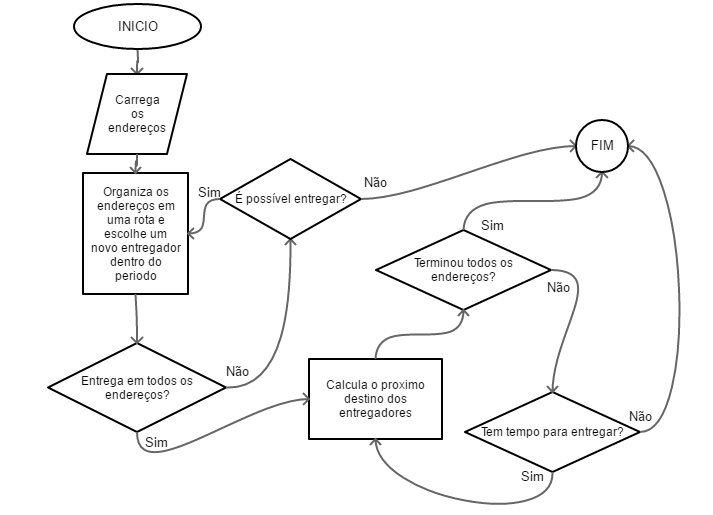
\includegraphics[keepaspectratio=true,scale=0.5]{ibagens/Fluxograma.png}}
    \captionof{figure}{Fluxograma macro do funcionamento do software.  }
    \label{fig:FluxoSoftware}
\end{minipage}

Sempre que é necessário calcular a rota, o modulo de GA é chamado. Considerando que um individuo é uma rota completa, gera uma população de varias rotas, onde a ordem da rota é aleatória somente mantendo o deposito fixo como primeiro endereço para criar a população inicial.
Para cada rota da população de indivíduos a seleção determina dois para a realização do cruzamento, onde endereços das duas rotas são trocados de forma a criar duas novas rotas mantendo o deposito sempre como inicial. A mutação é executada individual em cada rota, mudando de posição um ou mais endereços da rota, mas sempre 
mantendo o deposito como ponto inicial.

Depois que todas as rotas dos indivíduos da população foram modificados, agora é hora de verificar quais são os melhores, o que define isso é a função de aptidão, todos os parâmetros da rota são agrupados em um único numero e a rota que tem o menor numero é a melhor rota da população. O valor de aptidão é definido com a soma da distância entre todos os endereços da rota, mais o tempo de cada um dos trajetos com o tempo de espera e descarga.

A função de aptidão do GA considera o horário de saída como parâmetros inicial, com isso, utiliza o tempo dado pelo Google Maps entre os pontos e soma ao horário verificando se está dentro da janela de tempo do destino. Se o horário calculo for menor que o de abertura, é somado o tempo restante de espera. Se o horário for maior que o tempo de fechamento, é somado o tempo restante de espera até a abertura no próximo dia. Sempre que não chegar em um horário entra a janela de tempo, a penalidade é o tempo de espera, fazendo o tempo total ganhe mais peso no valor de aptidão. O Valor de aptidão final é a soma da distancia em metros do percurso passando por todos os pontos, com o tempo total em minutos.

O GA foi configurado com o numero de gerações em 200, tamanho da população em 1000, melhores indivíduos por geração em 20, probabilidade de cruzamento em 50\% e probabilidade de Mutação em 0,1\%.

Os testes foram configurados com um numero de 6 roteiros diferentes, endereços dentro da cidade de São Paulo e cidades próximas. Utilizando 6 tipos de mutação, sendo SM, IVM, IM, EM, DM e DIVM, e 2 tipos de cruzamento, sendo PBX e OBX.
Considerando o transito médio enviado pelo Google Maps, para poder demostrar o impacto do transito nos caminhos calculados.
Tudo será rodado 10 vezes e será retirada uma média do valor de aptidão, por que, cada vez que roda o GA a resposta da solução pode mudar, por ele não ser determinístico.

E uma base pré-definidas rotas, para prevenir possíveis problemas sera ignorado o transito atual. Ja que o mesmo altera dependendo das condições do clima ou horário do dia. Então utilizando o Google Maps, um cache inicial foi preparado e o software utiliza simulando uma buscar ao Google Maps, com isso, a informação é obtida mais rapidamente e sempre fixa para garantir a resposta pré-determinada do teste.

O fluxograma a baixo demostra o funcionamento do software utilizando o GA.

\begin{minipage}{\linewidth}
	\makebox[\linewidth]{
		\includegraphics[keepaspectratio=true,scale=0.5]{ibagens/GA.png}}
	\captionof{figure}{Fluxograma macro da integração com o GA.}
	\label{fig:FluxoGA}
\end{minipage}

\chapter{Implementação}
 
Nesse capitulo será apresentado mais aprofundadamente as tecnologias, ferramentas e métodos que foram utilizados para a implementação do algoritmo genético para busca de rota com janela de tempo.

\section{Tecnologias}

O software foi desenvolvido na linguagem C\# com Visual Studio 2017 com o Framework  .Net Core 2.2 compatível com Windows, Linux e MacOs para o Back-End e ReactJs para a interface de utilização.
Toda comunicação da interface com o calculador de rotas é por WebAPi Rest, onde são trocados dados em formato de Json.

\section{Estrutura do Projeto}

Para facilitar o entendimento inicial do projeto, é importante ter uma orientação de onde está cada parte de seu comportamento. A Solution do Visual Studio é divida em 4 projetos, onde eles são:

\subsection{PathFinder}
Projeto com função de utilização do software em geral, agrupamento informações de dados iniciais e organizando o retorno para a exibição.

\textbf{Program:} Implementação das união de todas as classes, executa a separação dos entregadores.

\textbf{Entregador:} Informação individual, armazena a rota completa do entregar e o genoma representante.

\textbf{TimeMeasure:} Configuração de registro/exibição do tempo de processamento.

\subsection{RouteGA}
Projeto de WebApi para a comunicação com a interface, seu objetivo é converter os dados recebidos pelo interface e chamar métodos do projeto \textbf{PathFinder}, convertendo o retorno para uma melhor estrutura que será exibida na interface.

\textbf{RouteController:} Implementação da comunicação da Api, recebe a requisição da interface, executa métodos do PathFinder e retorna uma lista da classe EntregadorViewModel para a interface.

\textbf{EntregadorViewModel:} Classe de retorno para a interface agrupando todas as informações da rota do entregador.

\textbf{LocalViewModel:} Classe de retorno para a interface agrupando todas as informações de um endereço.

\textbf{RotaViewModel:} Classe de retorno para a interface agrupando todas as informações de uma rota.

\textbf{RoteiroViewModel:} Classe de recebimento da interface agrupando todas as informações configuradas na interface para o calculo da rota.

\subsection{PathFinder.Routes}
Nesse projeto estão os algoritmos de comunicação com a  API Google Maps, classes para serialização dos retornos da API e classes para o agrupamento dos dados das rotas. Esse projeto é utilizado pelo genoma do GA para o recalculo das rotas

\textbf{GoogleMaps:} Classes de estrutura para serialização do Json de retorno da API do Google Maps.

\textbf{MapPoint:} Classe com informações do ponto de destino com latitude, longitude e janela de tempo para a entrega.

\textbf{Period:} Classe para a definição da janela de tempo.

\textbf{Route:} Classe para definição da origem e destino de uma rota, contendo o tempo e a distância entra os pontos.

\textbf{RouteMap:} Classe para a definição da rota completa e o deposito. A definição de cada caminho completo é controlado nessa classe. 

\textbf{SearchRoute:} Classe para a integração com a API do Google maps.

\subsection{PathFinder.GeneticAlgorithm}
Neste projeto são definidos todas as implementações referentes ao algoritmo genético, pela complexidade do algoritmo ele possui uma estrutura própria de pastas com algoritmos de seleção, cruzamento, mutação e a função de aptidão para definições e configurações de injeção de dependência.

\subsection{Abstraction}

Nesta pasta estão todos os arquivos a nível de abstração das etapas do algoritmo genético.

\textbf{ISelection}: Interface responsável por abstrair os algoritmos de seleção.

\textbf{IGenome}: Interface que tem como funcionalidade abstrair a definição de genoma.

\textbf{IFitness}: Interface que tem como objetivo abstrair o calculo de fitness.

\textbf{IMutate}: Interface que tem como objetivo abstrair os operadores de mutação.

\textbf{ICrossover}:  Interface que tem como objetivo abstrair os operadores de cruzamento.

\textbf{IRandom}: Interface que tem como objetivo abstrair a implementação de geração de números aleatórios.

\textbf{AbstractMutate}: Implementação base para operador de mutação.

\textbf{AbstractCrossover}: Implementação base para operador de cruzamento.

\subsection{Core}

\textbf{Enumerators}: Contem as definições de enumerações, usados para usar nomes bem definidos ao invés de números avulsos no código.

\textbf{RandomAdapter}: Implementação responsável por gerar números aleatórios, implementa IRandom.

\textbf{GASettings}: Arquivo responsável por carregar configuração estática de GA.

\textbf{Genome}: Classe responsável por representar o genoma no algoritmo de GA, implementa a IGenome.

\subsection{Selection}

Nesta pasta estão todas as implementações dos algoritmos de seleção.

\textbf{SelectionRouletteWheel}: Implementação de seleção roleta.

\subsection{Crossover}

Nesta pasta estão todas as implementações dos algoritmos de cruzamento.

\textbf{CrossoverOBX}: Implementação do operador de cruzamento OBX.

\textbf{CrossoverPBX}: Implementação do operador de cruzamento PBX.

\subsection{Mutation}

Nesta pasta estão todas as implementações dos algoritmos de mutação.

\textbf{MutateBitwise}: Implementação do operador de cruzamento Bitwise.

\textbf{MutateDIVM}: Implementação do operador de cruzamento DIVM.

\textbf{MutateDM}: Implementação do operador de cruzamento DM.

\textbf{MutateEM}: Implementação do operador de cruzamento EM.

\textbf{MutateIM}: Implementação do operador de cruzamento IM.

\textbf{MutateIVM}: Implementação do operador de cruzamento IVM.

\textbf{MutateSM}: Implementação do operador de cruzamento SM.

\subsection{Fitness}

Nesta pasta estão todas as implementações dos algoritmos de fitness.

\textbf{FitnessTimePath}: Implementação do fitness que considera o menor caminho e o tempo, para chegar no destino dentro da janela de tempo como a melhor solução.

\section{Funcionalidades}
O software é composto por funcionalidade individuais que podem ser utilizadas separadamente se necessário e também entender cada uma, ajuda a entender o software por completo.

\textbf{Integração com a API do Google Maps:} Usando a classe SearchRoute do projeto PathFinder.Routes é possível procurar rotas e endereços do Google Maps e obter informação de coordenadas geográficas de um ponto usando o endereço, calcular rota entre dos dois usando o endereço ou com as coordenadas geográficas, obter um mapa estático de um ou vários pontos.

\textbf{Algoritmos Genéticos} O modulo de GA poderia ser utilizado separadamente, porém é preciso o desenvolvimento da função de aptidão para o caso que ele será utilizado, o resto da estrutura funcionaria.